\documentclass{beamer}

\usepackage{kotex}
\usepackage{graphicx,psfrag,amsfonts,amsmath,amssymb}
\usepackage{multicol}
\usepackage{multirow}
% hyperlink
\usepackage{hyperref}
% code block option
\usepackage{listings}
\usepackage{xcolor}

\definecolor{codegreen}{rgb}{0,0.6,0}
\definecolor{codegray}{rgb}{0.5,0.5,0.5}
\definecolor{codepurple}{rgb}{0.58,0,0.82}
\definecolor{backcolour}{rgb}{0.95,0.95,0.92}

\lstdefinestyle{mystyle}{
	backgroundcolor=\color{backcolour},   
	commentstyle=\color{codegreen},
	keywordstyle=\color{magenta},
	numberstyle=\tiny\color{codegray},
	stringstyle=\color{codepurple},
	basicstyle=\ttfamily\footnotesize,
	breakatwhitespace=false,         
	breaklines=true,                 
	captionpos=b,                    
	keepspaces=true,                 
	numbers=left,                    
	numbersep=5pt,                  
	showspaces=false,                
	showstringspaces=false,
	showtabs=false,                  
	tabsize=2
}
\lstset{style=mystyle}

\usetheme{metropolis}

\usefonttheme[onlymath]{serif}	% 수식 설정!!

\title{Introduction to \LaTeX}
%\date{\today}
\date[Short Occasion]{Febrary 5, 2020}
\author{Hyunsung Kim}
\institute[Deptartment of Statistics]
	{Department of Statistics\\
	Chung-Ang University}

% A subtitle is optional and this may be deleted
%\subtitle{소제목}

%\author{F.~Author\inst{1} \and S.~Another\inst{2}}
% - Give the names in the same order as the appear in the paper.
% - Use the \inst{?} command only if the authors have different
%   affiliation.

%\institute[Universities of Somewhere and Elsewhere] % (optional, but mostly needed)
%{
%  \inst{1}%
%  Department of Computer Science\\
%  University of Somewhere
%  \and
%  \inst{2}%
%  Department of Theoretical Philosophy\\
%  University of Elsewhere}
% - Use the \inst command only if there are several affiliations.
% - Keep it simple, no one is interested in your street address.

%\date{Conference Name, 2013}
% - Either use conference name or its abbreviation.
% - Not really informative to the audience, more for people (including
%   yourself) who are reading the slides online

\subject{Introduction to \LaTeX}
% This is only inserted into the PDF information catalog. Can be left
% out. 

% If you have a file called "university-logo-filename.xxx", where xxx
% is a graphic format that can be processed by latex or pdflatex,
% resp., then you can add a logo as follows:

% \pgfdeclareimage[height=0.5cm]{university-logo}{university-logo-filename}
% \logo{\pgfuseimage{university-logo}}

% Delete this, if you do not want the table of contents to pop up at
% the beginning of each subsection:
%\AtBeginSubsection[]
%{
%  \begin{frame}<beamer>{Outline}
%    \tableofcontents[currentsection,currentsubsection]
%  \end{frame}
%}

% Let's get started
\begin{document}

\begin{frame}
  \titlepage
\end{frame}

\begin{frame}{Outline}
	\setbeamertemplate{section in toc}[ball unnumbered]
	\setbeamertemplate{subsection in toc}[ball unnumbered]
	\tableofcontents
	% You might wish to add the option [pausesections]
\end{frame}


\section{Tables}

\begin{frame}[containsverbatim]{How to make table?}
	\begin{lstlisting}[language=TeX, basicstyle=\tiny, caption=Table example code]
	\begin{table}[ht]
		\centering
		\begin{tabular}{ccc}       % alignment(c: center, l: left, r: right)
			\hline                   % horizontal line
			Var1 & Var2 & Var3 \\    % table elements(variable name + value)
			\hline
			1 & 2 & 3 \\
			4 & 5 & 6 \\
			7 & 8 & 9 \\
			\hline
		\end{tabular}
		\caption{Table example}    % caption
	\end{table}   \end{lstlisting}
\end{frame}

\begin{frame}{How to make table?}
	\begin{table}[ht]
		\centering
		\begin{tabular}{ccc}
			\hline
			Var1 & Var2 & Var3 \\ 
			\hline
			1 & 2 & 3 \\ 
			4 & 5 & 6 \\
			7 & 8 & 9 \\
			\hline
		\end{tabular}
		\caption{Table example}
	\end{table}
\end{frame}

\begin{frame}[containsverbatim]{Multiple columns and rows}
	\begin{multicols}{2}
	\noindent  
	$\triangleright$ Multiple rows
	\begin{lstlisting}[language=TeX, basicstyle=\tiny]
	\usepackage{multirow}
	
	\begin{table}[ht]
		\centering
		\begin{tabular}{ccc}
			\hline  
			Var1 & Var2 & Var3 \\ 
			\hline
			\multirow{2}{4em}{multi row} & 3 \\
			  & 5 & 6 \\
			7 & 8 & 9 \\
			\hline
		\end{tabular}
	\end{table}   \end{lstlisting}
	
	\columnbreak
	
	$\triangleright$ Multiple columns
	\begin{lstlisting}[language=TeX, basicstyle=\tiny]
	\begin{table}[ht]
		\centering
		\begin{tabular}{ccc}
			\hline 
			Var1 & Var2 & Var3 \\ 
			\hline
			1 & 2 & 3 \\
			4 & 5 & 6 \\
			7 & 8 & 9 \\
			\hline
		\end{tabular}
	\end{table}   \end{lstlisting}
	\end{multicols}
\end{frame}

\begin{frame}{Multiple columns and rows}
	\begin{multicols}{2}
		\noindent  
		$\triangleright$ Multiple rows
		\begin{table}[ht]
			\centering
			\begin{tabular}{ccc}
			\hline  
			Var1 & Var2 & Var3 \\ 
			\hline
			\multirow{2}{4em}{\textcolor{red}{multi row}} & 2 & 3 \\
			  & 5 & 6 \\
			7 & 8 & 9 \\
			\hline
		\end{tabular}
		\end{table} 
		
		\columnbreak
		
		$\triangleright$ Multiple columns
		\begin{table}[ht]
		\centering
		\begin{tabular}{ccc}
		\hline 
		Var1 & Var2 & Var3 \\ 
		\hline
		1 & \multicolumn{2}{c}{\textcolor{red}{multi col}} \\
		4 & 5 & 6 \\
		7 & 8 & 9 \\
		\hline
		\end{tabular}
		\end{table} 
	\end{multicols}
\end{frame}

\begin{frame}{Tables Generator}
	\begin{itemize}
		\item {
			GUI 형태로 값을 입력하는 방식
		}
		\item {
			입력된 테이블을 \textrm{\LaTeX} 코드로 변환해줌
		}
		\item {
			\href{https://www.tablesgenerator.com/}{\underline{Table Generator}}
		}
	\end{itemize}
\end{frame}

\begin{frame}{Tables Generator}
	\begin{figure}[h] %%% t: top, b: bottom, h: here
		\begin{center}
			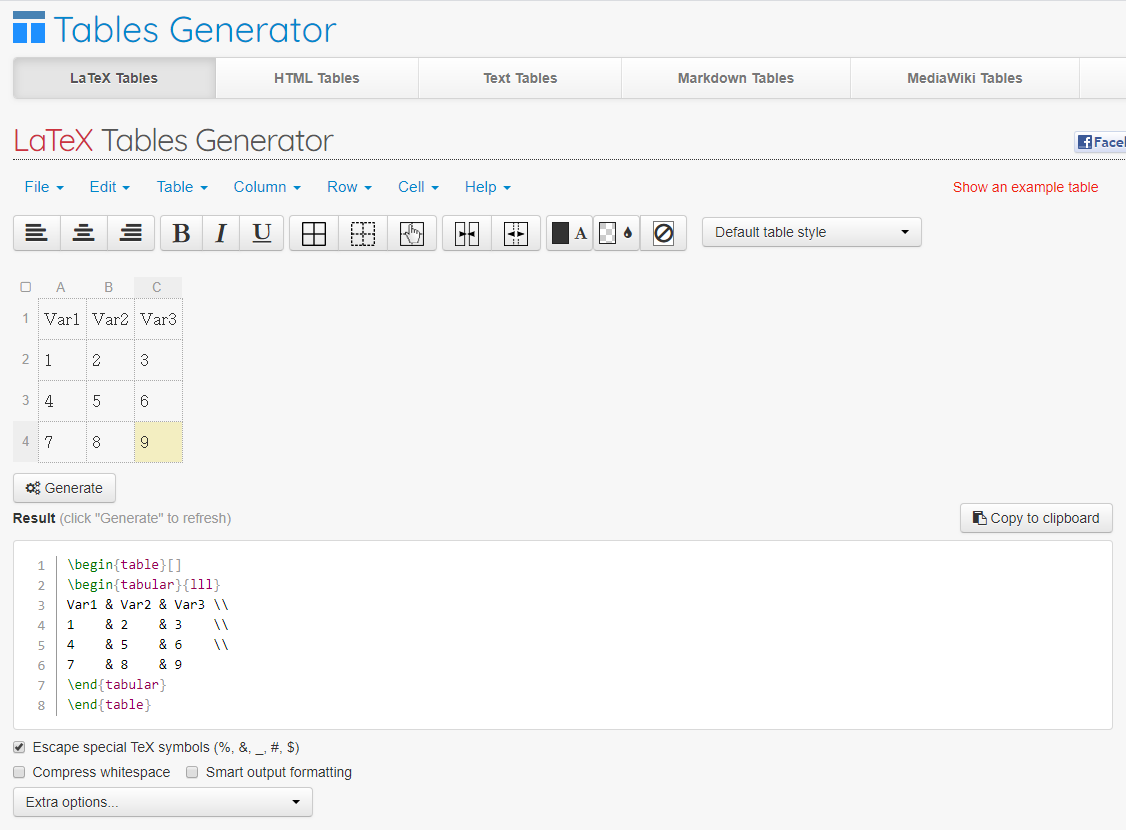
\includegraphics[width=0.7\linewidth]{img/table_generator.png}
		\end{center}
		\caption{Example table using Table Generator}
		\label{fig:long}
		\label{fig:onecol}
	\end{figure}
\end{frame}


%\subsection{\texttt{xtable} package}

\begin{frame}{\texttt{xtable} package}
	\begin{itemize}
		\item {
			\texttt{R}의 \texttt{dataframe} or \texttt{matrix} type을 \textrm{\LaTeX} 코드로 변환시켜주는 package
		}
		\item {
			"\texttt{xtable(df)}" 형식으로 사용
		}
		\item {
			\textrm{\LaTeX} 코드가 반환
		}
	\end{itemize}
\end{frame}

\begin{frame}{\texttt{xtable} package}
	\begin{figure}[h] %%% t: top, b: bottom, h: here
		\begin{center}
			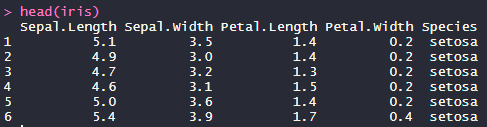
\includegraphics[width=0.9\linewidth]{img/xtable1.png}
		\end{center}
		\caption{The sample dataframe object}
		\label{fig:long}
		\label{fig:onecol}
	\end{figure}
\end{frame}

\begin{frame}{\texttt{xtable} package}
	\begin{figure}[h] %%% t: top, b: bottom, h: here
		\begin{center}
			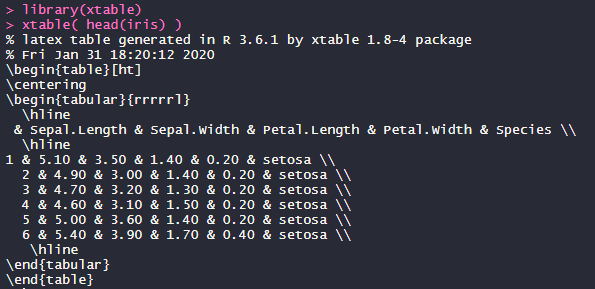
\includegraphics[width=0.9\linewidth]{img/xtable2.png}
		\end{center}
		\caption{Output of \texttt{xtable} function}
		\label{fig:long}
		\label{fig:onecol}
	\end{figure}
\end{frame}

\begin{frame}{\texttt{xtable} package}
	\begin{table}[ht]
		\centering
		\tiny
		\begin{tabular}{rrrrrl}
			\hline
			& Sepal.Length & Sepal.Width & Petal.Length & Petal.Width & Species \\ 
			\hline
			1 & 5.10 & 3.50 & 1.40 & 0.20 & setosa \\ 
			2 & 4.90 & 3.00 & 1.40 & 0.20 & setosa \\ 
			3 & 4.70 & 3.20 & 1.30 & 0.20 & setosa \\ 
			4 & 4.60 & 3.10 & 1.50 & 0.20 & setosa \\ 
			5 & 5.00 & 3.60 & 1.40 & 0.20 & setosa \\ 
			6 & 5.40 & 3.90 & 1.70 & 0.40 & setosa \\ 
			\hline
		\end{tabular}
		\caption{The table using output of \texttt{xtable} function}
	\end{table}
\end{frame}


\section{Figures}

\begin{frame}[containsverbatim]{How to input figures?}
	\begin{lstlisting}[language=TeX, basicstyle=\tiny, caption=Figure example code]
	\begin{figure}[h]   % t: top, b: bottom, h: here
		\begin{center}
			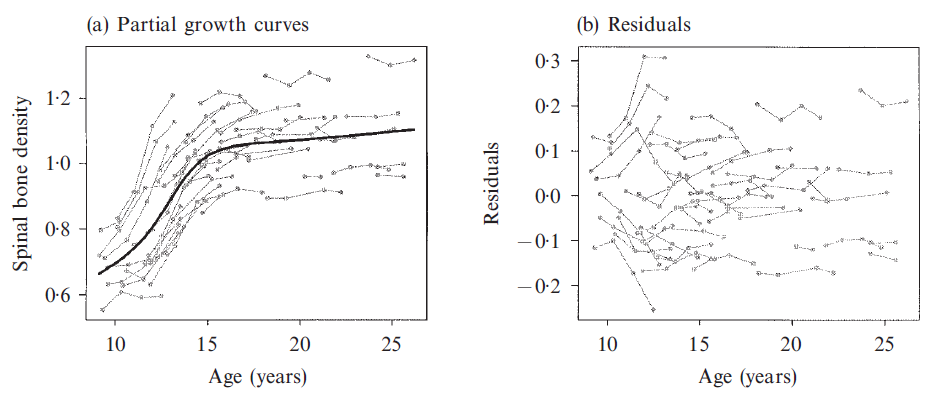
\includegraphics[width=0.7\linewidth]{img/figure.png}
		\end{center}
		\caption{Figure example}   % caption
		\label{fig:long}
		\label{fig:onecol}
	\end{figure}   \end{lstlisting}
\end{frame}

\begin{frame}{How to input figures?}
	\begin{figure}[h] %%% t: top, b: bottom, h: here
		\begin{center}
			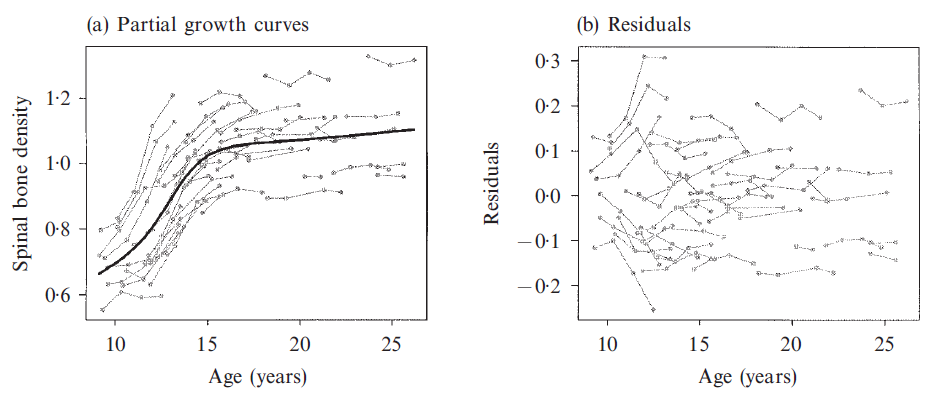
\includegraphics[width=0.7\linewidth]{img/figure.png}
		\end{center}
		\caption{Figure example}
		\label{fig:long}
		\label{fig:onecol}
	\end{figure}
\end{frame}



\section{Beamer Template}

%\subsection{Beamer Template}

\begin{frame}{What is Beamer?}
	\begin{itemize}
		\item {
			발표자료 형태의 \textrm{\LaTeX} 문서
		}
		\item {
			각 슬라이드에 내용을 넣는 방식으로 구성됨
		}
		\item {
			theme, color에 따라 다양한 양식 존재
		}	
		\item {
			\href{https://hartwork.org/beamer-theme-matrix/}{\underline{Beamer theme matrix}}
		}	
	\end{itemize}
\end{frame}

\begin{frame}{What is Beamer?}
	\begin{figure}[h] %%% t: top, b: bottom, h: here
		\begin{center}
			
\includegraphics[width=0.7\linewidth]{img/beamer_1.pdf}
		\end{center}
		\caption{Beamer example}
		\label{fig:long}
		\label{fig:onecol}
	\end{figure}
\end{frame}

\begin{frame}{What is Beamer?}
	\begin{figure}[h] %%% t: top, b: bottom, h: here
		\begin{center}
			
\includegraphics[width=0.7\linewidth]{img/beamer_2.pdf}
		\end{center}
		\caption{\texttt{Berlin} theme}
		\label{fig:long}
		\label{fig:onecol}
	\end{figure}
\end{frame}

\begin{frame}{What is Beamer?}
	\begin{figure}[h] %%% t: top, b: bottom, h: here
		\begin{center}
			
\includegraphics[width=0.7\linewidth]{img/beamer_3.pdf}
		\end{center}
		\caption{\texttt{Berlin} theme + \texttt{wolverine} colortheme}
		\label{fig:long}
		\label{fig:onecol}
	\end{figure}
\end{frame}

%\subsection{Example Code}

\begin{frame}[containsverbatim]{Example Code - Title}
	\begin{lstlisting}[language=TeX, basicstyle=\tiny, caption=Title code]
	\documentclass{beamer}      % document type
	
	\usetheme{Berlin}           % theme
	\usecolortheme{wolverine}   % color theme
	
	\title{Introduction to \LaTeX}   
	\date[Short Occasion]{Febrary 5, 2020}
	\author{Hyunsung Kim}
	\institute[Deptartment of Statistics]
	{Department of Statistics\\ Chung-Ang University}
	\subject{Introduction to \LaTeX}
	
	% create slides here
	\begin{document}
		
		% main title
		\begin{frame}
			\titlepage
		\end{frame}
		
	\end{document}   \end{lstlisting}
\end{frame}

\begin{frame}[containsverbatim]{Example Code - Slides}
	\begin{lstlisting}[language=TeX, basicstyle=\tiny, caption=Slides code]
	\begin{document}
	
		\section{Section 1}
		
		\subsection{Subsection 1}
		
		% slide 1
		\begin{frame}{Frame 1}
			\begin{itemize}
				\item {
					item 1
				}
				\item {
					item 2
				}
			\end{itemize}
		\end{frame}
	
	\end{document}   \end{lstlisting}
\end{frame}

\begin{frame}{Example Code - Slides}
	\begin{figure}[h] %%% t: top, b: bottom, h: here
		\begin{center}
			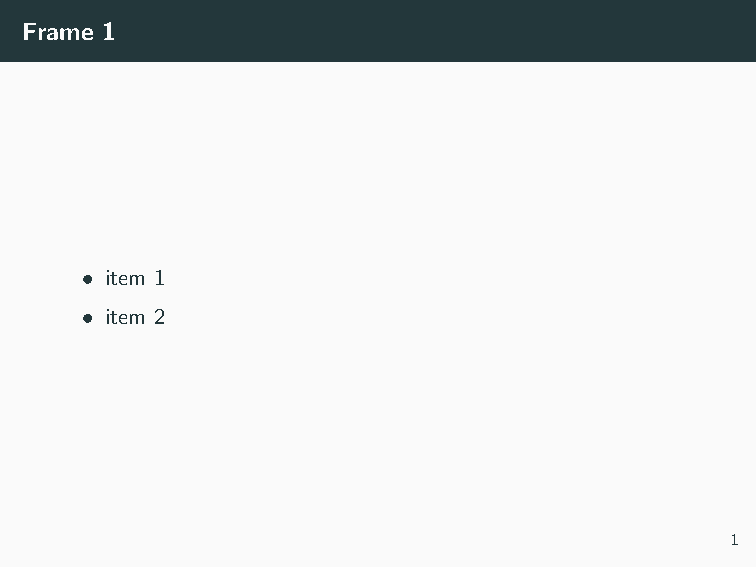
\includegraphics[width=0.7\linewidth]{img/beamer_item.pdf}
		\end{center}
		\caption{Slides example}
		\label{fig:long}
		\label{fig:onecol}
	\end{figure}
\end{frame}



\section{Useful Tips}

%\subsection{User defined command}

\begin{frame}{User defined command}
	\begin{itemize}
		\item {
			수식 작성시 반복해서 사용하게 되는 코드가 생김(bold체 등)
		}
		\item {
			\textrm{\LaTeX} 파일 상단에 축약해놓은 명령어를 지정해 놓고 사용하면 매우 편리!
		}
	\end{itemize}
\end{frame}

\begin{frame}[fragile]{Difference of codes}
	$$ \mathbf{B}_i \boldsymbol{\Theta} \mathbf{D} \boldsymbol{\Theta}^T \mathbf{B}^T_i $$
	\begin{multicols}{2}
	\noindent  
	$\triangleright$ Original code
	\begin{lstlisting}[language=TeX]
	$$ 
	\mathbf{B}_i \boldsymbol{\Theta} \mathbf{D} \boldsymbol{\Theta}^T \mathbf{B}^T_i 
	$$  \end{lstlisting}
	
	\columnbreak
	
	$\triangleright$ User defined code
	%\vspace{-0.154cm}
	\begin{lstlisting}[language=TeX]
	$$ 
	\bB_i \bTheta \bD \bTheta^T \bB^T_i 
	$$ \end{lstlisting}
	\end{multicols}
\end{frame}

\begin{frame}[fragile]{User defined command}
	$\triangleright$ 다음과 같이 정의하여 사용하면 됨
	
	\begin{lstlisting}[language=TeX]
	\def \bY { \mathbf{Y} }
	\def \bB { \mathbf{B} }
	\def \bI { \mathbf{I} }
	\def \bD { \mathbf{D} }
	\def \bbeta { \boldsymbol{\beta} }
	\def \btheta { \boldsymbol{\theta} }
	\def \bTheta { \boldsymbol{\Theta} }
	\def \balpha { \boldsymbol{\alpha} }  \end{lstlisting}
\end{frame}


%\subsection{Code block}

\begin{frame}{Code block}
	\begin{itemize}
		\item {
			코드를 같이 제출하는 과제가 있는 강의를 들을 때 유용 (통계계산론, 데이터마이닝 등)
		}
		\item {
			단순 코드 복붙보다 깔끔하게 정리 가능
		}
		\item {
			코드를 \textrm{\LaTeX} 파일에 직접 넣지 않고 코드 파일을 첨부하여 사용 가능
		}
		\item {
			\href{https://www.overleaf.com/learn/latex/Code_listing}{\underline{Reference}}
		}
	\end{itemize}
\end{frame}

\begin{frame}{Build directory}
	\begin{itemize}
		\item {
			\textrm{\LaTeX} 파일 compile시, \texttt{pdf} 뿐만 아니라 다른 파일들이 같이 생김
		}
		\item {
			임시 파일들이 따로 폴더에 들어가도록 설정할 수 있음
		}
		\item {
			\texttt{TeXstudio} + \texttt{Miktex} 기준의 설정 방법
		}
		\item {
			\texttt{PdfLaTeX}의 명령어를 다음과 같이 수정하여 설정 가능 \\
			\texttt{pdflatex.exe -synctex=0 -interaction=nonstopmode --aux-directory=build \%.tex}
		}
	\end{itemize}
\end{frame}

\begin{frame}{How to config Build directory?}
	\begin{figure}[h] %%% t: top, b: bottom, h: here
		\begin{center}
			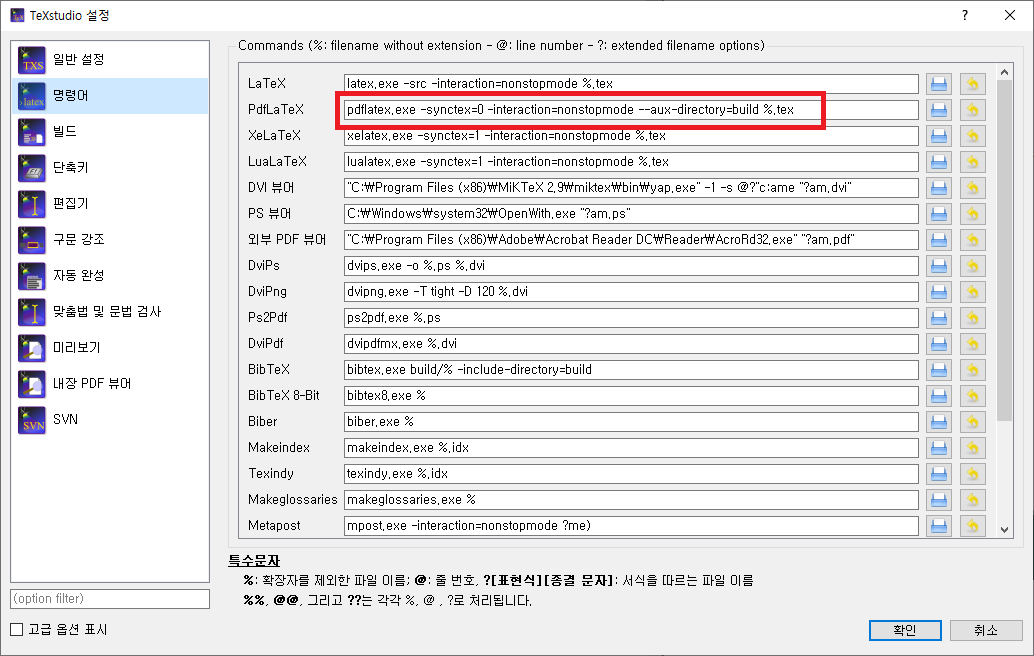
\includegraphics[width=0.8\linewidth]{img/texstudio_config.png}
		\end{center}
		\caption{Settings in texstudio}
		\label{fig:long}
		\label{fig:onecol}
	\end{figure}
\end{frame}

\begin{frame}{Before configuration}
	\begin{figure}[h] %%% t: top, b: bottom, h: here
		\begin{center}
			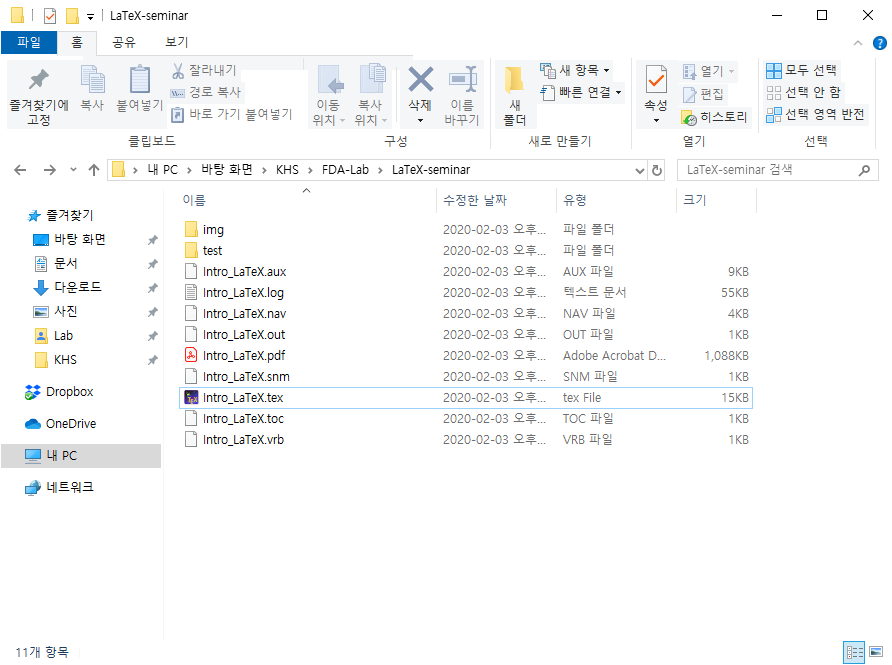
\includegraphics[width=0.8\linewidth]{img/config_before.png}
		\end{center}
		\caption{Before configuration}
		\label{fig:long}
		\label{fig:onecol}
	\end{figure}
\end{frame}

\begin{frame}{After configuration}
	\begin{figure}[h] %%% t: top, b: bottom, h: here
		\begin{center}
			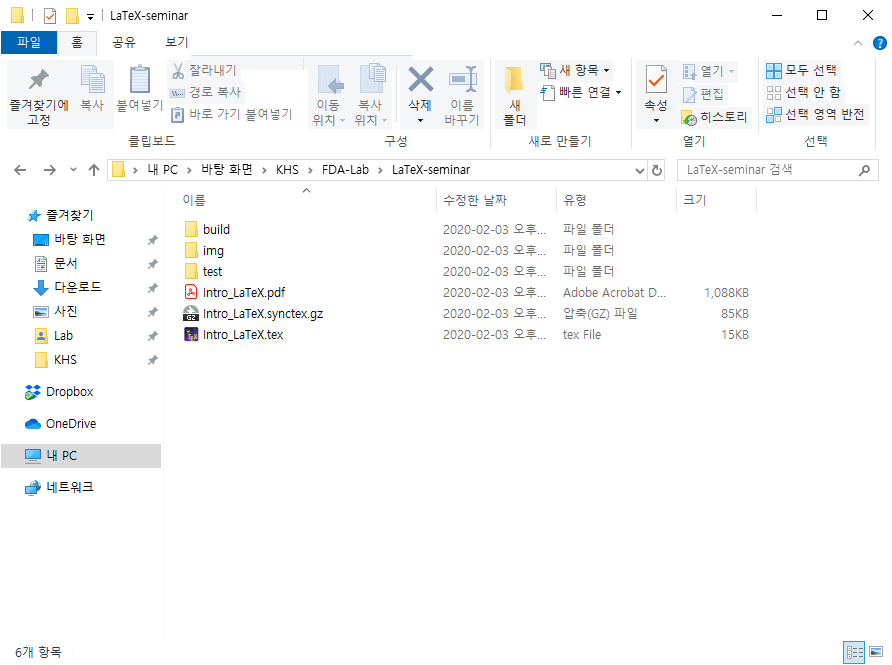
\includegraphics[width=0.8\linewidth]{img/config_after.png}
		\end{center}
		\caption{After configuration}
		\label{fig:long}
		\label{fig:onecol}
	\end{figure}
\end{frame}

%\subsection{Rmarkdown to Beamer}

\begin{frame}{Rmarkdown to Beamer}
	\begin{itemize}
		\item {
			\texttt{Rmarkdown}으로 \textrm{\LaTeX} 문서 작성 가능 \\
			(단, \textrm{\LaTeX} 설치되어 있는 경우만 가능)
		}
		\item {
			\texttt{Markdown} 문법 + \textrm{\LaTeX} 혼용 가능
		}
		\item {
			\href{https://github.com/statKim/TIL/blob/master/R/R\%20markdown\%EC\%97\%90\%EC\%84\%9C\%20Beamer(Tex)\%20\%EC\%8A\%AC\%EB\%9D\%BC\%EC\%9D\%B4\%EB\%93\%9C\%20\%EB\%A7\%8C\%EB\%93\%A4\%EA\%B8\%B0.md}{\underline{Reference}}
		}
	\end{itemize}
\end{frame}



\begin{frame}
	\begin{center}
		\huge
		감사합니다!
	\end{center}
\end{frame}


\end{document}


